\documentclass[tikz,border=3pt]{standalone}
\usepackage[T1]{fontenc}
\usepackage{lmodern}
\usetikzlibrary{arrows.meta,positioning,calc}
\definecolor{ink}{HTML}{182C3C}
\definecolor{teal}{HTML}{007F80}
\definecolor{amber}{HTML}{B46D20}
\definecolor{mist}{HTML}{EEF4F5}
\definecolor{pale}{HTML}{F6F0E5}
\begin{document}
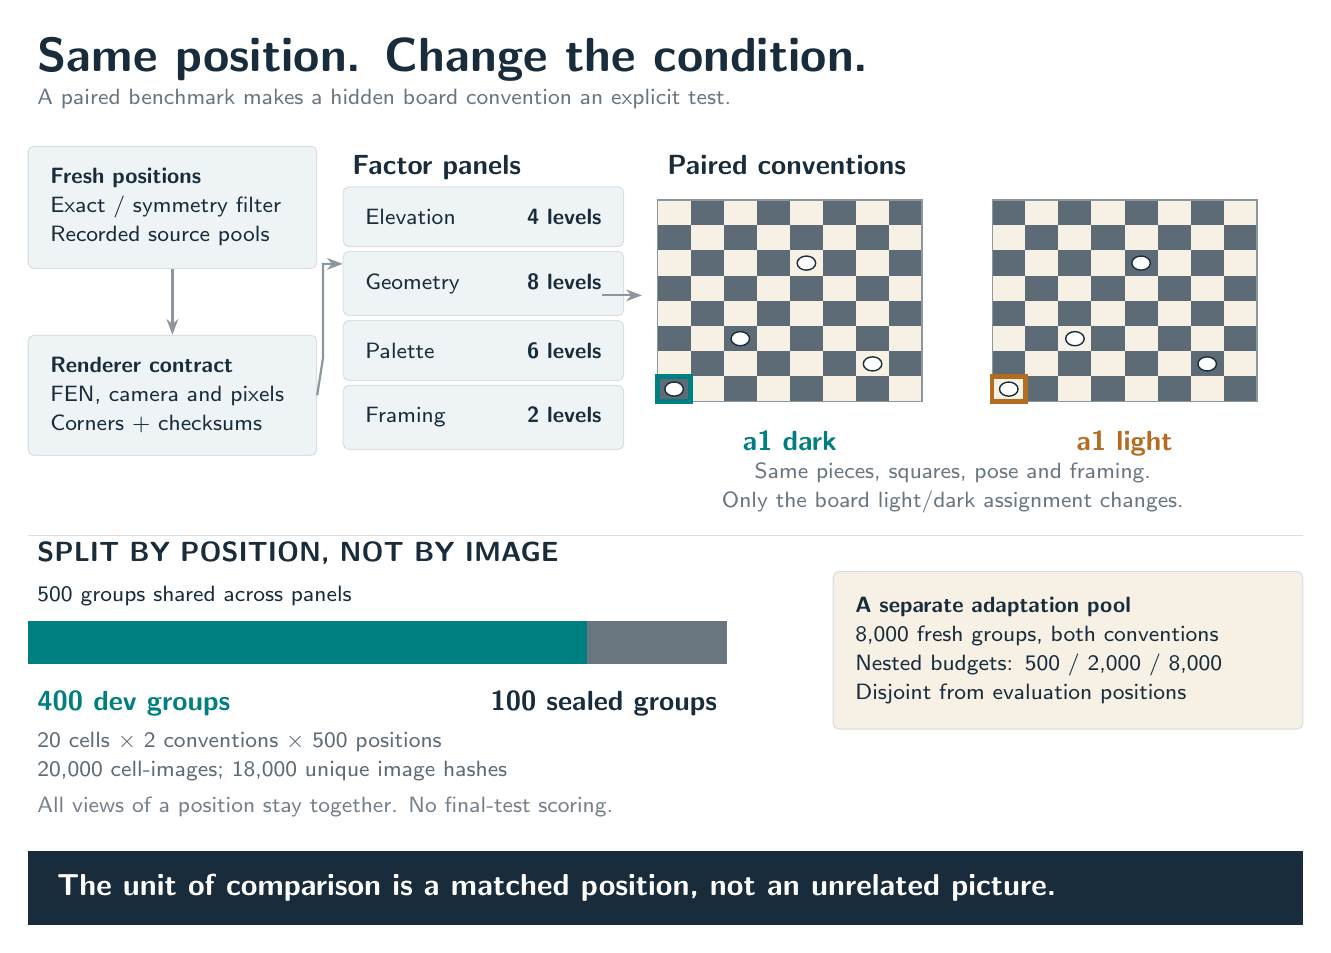
\begin{tikzpicture}[x=1cm,y=1cm,font=\sffamily\fontsize{8.5}{10.5}\selectfont,text=ink,
  box/.style={rounded corners=2pt,draw=ink!15,fill=mist,inner sep=8pt,align=left},
  link/.style={-{Stealth[length=2mm]},line width=.8pt,draw=ink!50}]
\path[use as bounding box] (0,0) rectangle (16.2,11.4);
\node[anchor=west,font=\sffamily\bfseries\fontsize{18}{20}\selectfont] at (0,11.0) {Same position. Change the condition.};
\node[anchor=west,text=ink!65] at (0,10.5) {A paired benchmark makes a hidden board convention an explicit test.};
% receipt: evidence/benchmark_v2/design.complete.json; benchmark_groups, adaptation_groups
\node[box,text width=3.1cm,minimum height=1.45cm,anchor=north west] (source) at (0,9.9) {\textbf{Fresh positions}\\Exact / symmetry filter\\Recorded source pools};
\node[box,text width=3.1cm,minimum height=1.45cm,anchor=north west] (contract) at (0,7.5) {\textbf{Renderer contract}\\FEN, camera and pixels\\Corners + checksums};
\draw[link] (source.south)--(contract.north);
\node[anchor=north west,font=\sffamily\bfseries] at (4.0,9.9) {Factor panels};
% receipt: evidence/benchmark_v2/benchmark.summary.json; cells keys by factor
\foreach \yy/\label/\count in {9.0/Elevation/4,8.15/Geometry/8,7.3/Palette/6,6.45/Framing/2}{
 \node[box,anchor=west,text width=3.0cm,minimum height=.6cm] at (4.0,\yy) {\label\hfill\textbf{\count\ levels}};
}
\draw[link] (contract.east)--(3.75,7.2)--(3.75,8.4)--(4.0,8.4);
\node[anchor=north west,font=\sffamily\bfseries] at (8.0,9.9) {Paired conventions};
% The squares/pieces below are a vector illustration, not experimental frames.
% receipt: evidence/docs/BENCHMARK_V2_2026-09-10.md; paired a1_dark/a1_light contract
\foreach \off/\parity/\accent/\label in {8.0/0/teal/a1 dark,12.25/1/amber/a1 light}{
 \begin{scope}[shift={(\off,6.65)},x=.42cm,y=.32cm]
  \foreach \x in {0,...,7}{\foreach \y in {0,...,7}{
   \pgfmathtruncatemacro{\v}{mod(\x+\y+\parity,2)}
   \ifnum\v=0 \fill[ink!70] (\x,\y) rectangle +(1,1);
   \else \fill[pale] (\x,\y) rectangle +(1,1);\fi
  }}
  \draw[ink!50,line width=.5pt] (0,0) rectangle (8,8);
  \foreach \xx/\yy in {.5/.5,2.5/2.5,6.5/1.5,4.5/5.5}{
   \filldraw[fill=white,draw=ink,line width=.5pt] (\xx,\yy) circle (.28);
  }
  \draw[\accent,line width=1.6pt] (0,0) rectangle (1,1);
 \end{scope}
 \node[anchor=north,font=\sffamily\bfseries,text=\accent] at (\off+1.68,6.4) {\label};
}
\draw[link] (7.3,8.0)--(7.8,8.0);
\node[align=center,text=ink!65,text width=7.4cm] at (11.75,5.55) {Same pieces, squares, pose and framing.\\Only the board light/dark assignment changes.};
\draw[ink!15] (0,4.95)--(16.2,4.95);
\node[anchor=west,font=\sffamily\bfseries] at (0,4.72) {SPLIT BY POSITION, NOT BY IMAGE};
% receipt: evidence/benchmark_v2/design.complete.json; benchmark_groups=500
\node[anchor=west] at (0,4.18) {500 groups shared across panels};
% receipt: evidence/benchmark_v2/benchmark.summary.json; cells, partitions, unique_image_hashes
\fill[teal] (0,3.32) rectangle (7.1,3.86);
\fill[ink!65] (7.1,3.32) rectangle (8.88,3.86);
\node[anchor=north west,text=teal,font=\sffamily\bfseries] at (0,3.1) {400 dev groups};
\node[anchor=north east,text=ink,font=\sffamily\bfseries] at (8.88,3.1) {100 sealed groups};
\node[anchor=north west,text=ink!70,align=left] at (0,2.58) {20 cells $\times$ 2 conventions $\times$ 500 positions\\20,000 cell-images; 18,000 unique image hashes};
\node[box,fill=pale,text width=5.4cm,anchor=north east,minimum height=2.0cm] at (16.2,4.5) {\textbf{A separate adaptation pool}\\8,000 fresh groups, both conventions\\Nested budgets: 500 / 2,000 / 8,000\\Disjoint from evaluation positions};
% receipt: evidence/benchmark_v2/adaptation.complete.json; images=16000
\node[anchor=west,text=ink!60] at (0,1.5) {All views of a position stay together. No final-test scoring.};
\fill[ink] (0,0) rectangle (16.2,.94);
\node[anchor=west,text=white,font=\sffamily\bfseries\fontsize{11}{13}\selectfont] at (.25,.48) {The unit of comparison is a matched position, not an unrelated picture.};
\end{tikzpicture}
\end{document}
